\documentclass[a4paper, english, 12pt]{article}

\usepackage[utf8]{inputenc}
\usepackage[T1]{fontenc}
\usepackage{graphicx}
\usepackage{babel}
\usepackage{amsmath,amsfonts,amssymb}

\title{An Introduction to Ontology\\ INF219\\ University of Bergen}
\date{\today}
\author{Teis Lindemark}

\begin{document}
\maketitle{}
\tableofcontents{}
\pagebreak
\begin{abstract}
    \centering
    \begin{minipage}{0.7\textwidth}
	An ontology is a detailed model of a part of the reality which is built up on the facts and relations we know about in a domain. Ontologies are useful because they often defines a common vocabulary in a domain, that make collaboration between researchers easier and it also enable the reuse of the domain of knowledge. Ontology engineering is about developing an ontology, which is an iterativ process. The section about evaluating an ontology, covers different approaches and methodologies. At the end, there are examples of practical usage of ontologies.
    \end{minipage}
\end{abstract}

\section{Forword}
This report is a part of the course INF219 at University of Bergen. The work is an introduction to ontology as a pre-work to a potential master thesis topic. The aim of this report is to give a general introduction to ontologies and the main topics related to this. It covers the main parts of ontology to give a meaningful introduction to the topic.

\section{What is an ontology?}
The word ontology originally came from philosophy, and has been adopted in many other field of business. In the philosophical domain, the word ontology means a branch of metaphysics concerned with the study of existence.In the scientific and information "world" there are several definitions of the word ontology. Tom Gruber's definition: "An ontology is a specification of a conceptualization." or "Ontologies are specifications of a relational vocabulary". Wikipedia have these definition: "An ontology is a data model that represents a set of concepts within a domain and the relationships between those concepts".\cite{website:wikipediaontology} An ontology is aso a formal description of classes (sometimes called concepts) in a domain of discourse, each class has properties describing different features and attributes of the classes, and restriction on facets. There are a set of individual instances of classes that compose a knowledge base.\cite{website:standford} An ontology is developed or produced to set a structure of data for other programs to use.

In all these definitions for the same word, there are a lot of complex words like conceptualization, domain and 'relational vocabulary'. Conceptualization, we can say is an abstract, simplified picture of the world we want to be represented for some reason. A domain is a part of the world, like cats is a part of the pets world for example.

From this, an ontology is a detailed model of a part of the reality which is build up on the facts and relations that we know (knowledge domain). The W3C organization describe ontology: "An ontology defines the terms used to describe and represent an area of knowledge".\cite{website:whatontology}

\section{Why develop an ontology?}
In the World-Wide Web, there has started to be common to develop ontologies to categorization of products. There are also more and more fields that have developed standarized ontologies to make it easier to share a common understanding of the information. In the World-Wide Web, the WWW Consortium (W3C)\footnote{International community where member organizations, full-time staff and the public collaborate to develop Web-standards \cite{website:w3c}} is developing the "Resource Description Framework", that is a language for encoding knowledge on Web pages. This makes it understandable for electronic agents that is searching for information. An ontology is useful because it defines a common vocabulary in the field so different researchers easier can share information in a domain and the understanding is better. The United Nations Development Program and Dun \& Bradstreet have developed the UNSPSC ontology which contain terminology for products and services (http://www.unspsc.org/).

By developing an ontology it also enable the reuse of the domain of knowledge. If some researchers develop an ontology, other researchers that are developing or need an ontology that is similar, can just reuse it.

Developing an ontology of the domain is often not the aim, but developing an ontology to define a set of data and the structure for other programs to use. That can be software agents or web applications.\cite{website:standford}

\section{Ontology engineering}
The first thing to know about ontology engineering is that there is not one "correct" way to developing ontologies. Some important rules in ontology design to help making the design decisions is:
\begin{itemize}
	\item There is more than one way to model a domain. There are always alternatives and the best solution depends on the application that you should develop an ontology for.
	\item Ontology engineering is an iterative process \footnote{A process for arriving at a decision by repeating rounds of analysis.}
	\item Concepts in the ontology are to be close to objects and relationships in the domain of interest.
\end{itemize}

To start developing an ontology, it is best to define its domain and scope. To do that, it is useful to have a couple of questions in mind:
\begin{itemize}
	\item Which domain will the ontology cover?
	\item What are the usage of the ontology?
	\item What kind of questions is the information in the ontology meant to give an answer?
	\item Who is the users and the maintainers of the ontology?
\end{itemize}
These questions may change in the ongoing work with the ontology developing. That is the reason developing an ontology is an iterative process.

It is necessary is to look at ontologies already existing, to check if it is possible to reuse an existing ontology. There are reusable ontologies on the web and in the literature. There is important to have in mind that it probably no one of the existing ontologies will fit perfectly, but there are a lot of existing ontologies available in electronic and the task of translating an ontology from one formalism to another is usually not a difficult one.

It will be needed to write down exact terms that is needed to make statements. Some questions that can be helpful are: "What are the terms we want to talk about?", "What properties do those terms have?" etc. Graninger and Fox called it competences questions. This will be helpful in the next step where the classes and the class hierarchy are defined.

The classes and the class hierarchy has to be defined. There are different approaches to do this and they will end up with more and less the same result. There are three main approaches, top-down, bottom-up and a combination. Which of the approaches that is chosen is up to the developer of the ontology.
\begin{itemize}
	\item A {t\bf op-down approach} development starts at the most general classes in the domain and work down with more and more specific classes.
	\item A{\bf  bottom-up approach} development is the opposite of the top-down approach where you start with the classes that is most specific and working up to the most general classes.
	\item A {\bf combination} development combine these two approaches, top-down and bottom-up.
\end{itemize}

Figure \ref{fig:example_classhierachy} gives a possible breakdown of classes and sub-classes in the class hierarchy wholes. The figure show the most general classes (top level) and down (middle level and bottom level).

\begin{figure}[htb]
	\centering
	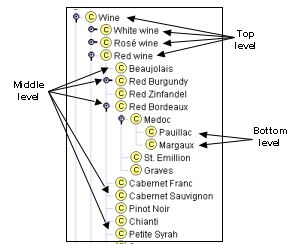
\includegraphics[scale=0.75]{figures/classhierarchical.jpg}
	\caption{Example class hierarchy from an example with wine.\cite{website:standford}}
	\label{fig:example_classhierachy}
\end{figure}

It is not enough with dividing only the classes to get the answers that is pointed out in the first step, it is also necessary to define properties to the classes. For each property we define, we have to define which class the property contain. The subclasses of a class inherits the properties from that class and a property should also be attached to the most general class that can have that property.

Each property also have to be defined a type. Examples of different types can be: string, number, boolean, enumerated and instance. String is a text string. Number can be float or integer. The boolean type is just a true/false value or it can be 1/0, where 1 is true and 0 is false. Enumerated is a list of allowed values. Instance allow to definition of relationship between individuals.

The last step is to create the instances. To define an individual instance of a class, there are three steps:
\begin{enumerate}
	\item Choosing a class
	\item Creating an instance of the chosen class
	\item Filling in the properties for the chosen instance.
\end{enumerate}
\cite{website:standford}

\section{How to evaluate an ontology?}

\subsection{Approaches}
There are two different ways to evaluate an ontology, qualitative and quantitative approach. With a qualitative approach, it is difficult to know who the right persons to evaluate are. There could be the user that should use the system, there could be the domain expert or someone else who has competence at the area. It is also hard to develop automated tests to the ontologies. The quantitative evaluating of an ontology consider the effectivity of an ontology in a context of an application and is the most common one. There is one more approach that concerns the congruence between an ontology and a domain of knowledge. When a new developed ontology is used together with an existing "equal" ontology at a domain of knowledge, and the results differs, it is not obvious to find the causes. It can be that the corpus is inappropriate or there is a real difference in the knowledge showed in the corpus and the existing ontology.\cite{brewster}

\subsection{Methodologies}
The methodologies for evaluating an ontology is not the same as methodologies for ontology engineering. In evaluation, they provide a framework for defining well-suited methods for evaluating ontologies. Here I will present two ontology-evaluating methodologies: \cite{yu}

\subsubsection{OntoClean}
OntoClean is a methodology for analyzing ontologies that is based on formal, domain-independent properties of classes. By using OntoClean, can help an ontology to meet the evaluation criterion of correctness. Here correctness means if the entities and properties in an ontology correct give a picture of the world that is modeled. The way OntoClean does this is by introducing meta-properties  to capture different characteristics of classes and constraints by those meta-properties. That help to consider the correct usage of the subsumption relation between classes in an ontology.

The meta-properties in OntoClean is identity, unity, rigidity and dependence. Identity is normal in many fields, as metaphysics and database conceptual modeling. In this cases there is an accepted practice to make a primary key for the rows in a table. Each row has a unique primary key, so if "more" than one row have the same primary key, they are the same row. In OntoClean, identity criteria are some classes of entities, called sortals. This is a class all of whoes instances that are identified in the same way. In information systems, criteria like this are often outer, like universally unique id, but in the ontology world, this is not interesting. Identity criteria should be informative and should be helping the users to understand what a class means. The next meta-properties is unity, that are some properties that only contains of individuals that are wholes. In OntoClean, wholes are individuals all of whose parts are related to each other, and only to each other, by some distinguished relation. The third meta-properties can be described by an example; If I have long hair one day and then take a cut off the hair the next day, yet I am the same entity at both times. How is it possible for me to be the same if I have changed? This is one of many logical approaches to this dilemma, the most usual is to look at some properties to be essential and an essential property of an entity cannot change, and there are for these kind of properties Leibniz's law hold. The properties of an entity that are non-essential can change, but they cannot be involved in the identity. The last meta-property in the OntoClean methodology is dependence. This mean that if a property should be dependent, each of the instances of it implies the existence of another entity.
\cite{yu,website:wikipediaontoclean}

\subsubsection{OntoMetric}
The OntoMetric methodology is using application constraints as the basis for ontology selection. In OntoMetric there are five dimentions at the top level of the taxonomy, that are: content, language, methodology that is used to develop the ontology, tools that are used to develop the ontology and the cost to utilise the ontology. There are associated a set of factors to each of the dimension and for each factor. To get the characteristics it is needed to take this from existing work and include design qualities, ontology evaluation criteria, cost and language characteristics. The OntoMetric methodology use this steps:
\begin{enumerate}%Utdyp mer!
	\item Analyse project aim
	\item Obtain a customised a multilevel tree of characteristics (MTC). This should be based on a set of objectives from the project aim.
	\item Weight up each characteristics against each other. Two and two characteristics are weighted against each other to show the importance of one characteristics over another. A given weight wt is given for each characteristics to assign them against each other. A comparison matrix is made of the pairwise comparison and the eigenvectors are calculated from this matrix.
	\item Assign linguistic score for each characteristics of a candidate ontology. 
	\item Select the most suitable ontology. How close the characteristics of each candidate ontology is evaluated. This is showed by comparing vectors of the weight wt and wc of the candidate ontology c and the modified taxonomy of characteristics in the customized MTC.
\end{enumerate}
There are some limitations in the OntoMetric methodology too, like that the determining the customised MTC for the ontology selection is depending at the manual specification, and this can be subjective or inconsistent. The list of characteristics that is used for evaluating content is limited. The linguistic scale is up to the user to assign values of an ontology characteristics, so there is not used specific measurements. The OntoMetric methodology can only be used to check which ontology that is best fit from a set of candidates ontologies. \cite{yu}

\section{Practical usage}
Every day, we are surrounded by usage of ontologies. It is used in the background when we are on the World Wide Web at our computer or phone. Ontologies are in use everywhere. In this general introduction, there are chosen to examples where it can be useful to use an ontology. Both in the semantic web and in data integration, there could be huge set of data, so the domain of knowledge will then be large. Using ontologies to structuring the domain will be useful.

\subsection{Semantic Web}
The Semantic Web is a "web of data" that makes it easier for machines to understand the semantics of information on the World Wide Web. More precise it extends the network of human-readable web pages by including machine-readable metadata about pages and in which way the pages are related to each other, starting automated agents to access the Web smarter and perform tasks in place of the users. The term Semantic Web is also used specifically to refer to the format and technologies that activates it. The technologies that activates the semantic web process contain the "Resource Description Framework (RDF)", and notations such as RDF Schema and the Web Ontology Language, that all of them gives a formal description of concepts, terms and relationships within a given knowledge domain.\cite{website:wikipediasemanticweb}

The Web Ontology Language (OWL) is a knowledge representation language for authoring ontologies. OWL is approved by the W3C organization, and has getting academic, medical and commercial interest.

\subsection{Data integration}
Data integration includes combining data from different sources and give the user a view of those data. This process is widely used both commercial and in scientific purposes. In more and less all the information systems today, the data is coming from more than one data source. In web applications for example where a user can request a query variety  of information about cities such as weather forecast, hotels, car rentals and so on. To have all this information in one database, will duplicate the information. With data integration the solution can construct a virtual schema, to best model the answer the user want. Then the developers design adapters for each data source. The adapters just transform the local query request into  an an procesed form for the data-integration solution. \cite{website:wikipediadataintegration}

To make data integration possible in an easy way, it is very helpful to have standardized data. Standards defines the interface of a software system, for example standards define the syntax and semantics of a programming language or even a data model. Today, database systems are complex and are very often created of multiple independently parts that need to collaborate together. This is going to data integration where application often use multiple data sources. Standards that are developed by standards organizations or by industry groups are formal standards, but dominant products can be general accepted as a "de facto standards" without any formal standards process. \cite{database}

As mentioned in section 2, ontology is a model of a domain. The ontology is often used to make a model of the domain and then use the model to create a database. %UTDYP

\section{Conclusion}
In this report, I give a general introduction to ontologies by describing some main topics. I describe the origin of the word "ontology" and give some main definitions of the word for our use. The motivation, or needs, for developing and using ontologies is a main part and both practical use and reasons for use are treated. I have given ways to engineer better ontologies and ways to evaluate ontologies. In the end I give two examples for practical usage. I have read and learned a lot about ontologies. A main understanding is that no 100\% correct ontology is, or will be, created.The more useful an ontology would be, the closer to impossible it is going to be make it.

\bibliographystyle{plain}
\bibliography{bib}

\end{document}